%=====================================================================
%  A Digital-Twin and Physical-Watermarking Testbed for Multi-Layer
%  Intrusion Detection in SCADA Systems
%
%  Compiles on Overleaf out of the box (pdfLaTeX, IEEEtran).
%  Figures are in ./figures/  (4 real screenshots as .jpg).
%  The architecture diagram, the data-flow flowchart and the results
%  chart are drawn with TikZ/pgfplots, so no extra image files are needed.
%=====================================================================
\documentclass[conference]{IEEEtran}
\IEEEoverridecommandlockouts

\usepackage{cite}
\usepackage{amsmath,amssymb,amsfonts}
\usepackage{graphicx}
\usepackage{booktabs}
\usepackage{array}
\usepackage{xcolor}
\usepackage{tikz}
\usepackage{pgfplots}
\usepackage[hidelinks]{hyperref}
\usetikzlibrary{shapes.geometric,arrows.meta,positioning,calc,fit,backgrounds}
\pgfplotsset{compat=1.17}

% ---- theme colours (match the platform's dark/orange HMI) ----
\definecolor{acc}{HTML}{E0572F}      % orange accent
\definecolor{lnet}{HTML}{3B82C4}     % network layer
\definecolor{lproc}{HTML}{8B5CF6}    % process layer
\definecolor{ltwin}{HTML}{1F9D5A}    % twin layer
\definecolor{lwm}{HTML}{C79400}      % watermark layer
\definecolor{slate}{HTML}{334155}
\definecolor{lightgray}{HTML}{EEF1F5}

\begin{document}

\title{A Digital-Twin and Physical-Watermarking Testbed\\ for Multi-Layer Intrusion Detection in SCADA Systems}

\author{%
\IEEEauthorblockN{S. Saurabh Krishnan, \quad Hemant Bhupesh, \quad Sanjai S, \quad Nitesh V. M.}
\IEEEauthorblockA{\textit{Amrita Vishwa Vidyapeetham}\\
Coimbatore, India}
}

\maketitle

\begin{abstract}
Industrial supervisory control and data acquisition (SCADA) systems are increasingly targeted by attacks that falsify sensor telemetry or inject unauthorised control commands. Conventional network intrusion detection observes only the communication layer and is therefore blind to attacks that manipulate a field device directly. This paper presents a fully simulated, reproducible cyber-physical security testbed built around a liquid-metal boiler plant, and uses it to evaluate a defence that combines four complementary detection layers---network, process, an independent digital twin, and physical watermarking---fused by a correlation engine. The digital twin integrates its own physics model with datasheet parameters and a gated measurement-fusion rule, so a falsified reading produces a growing, detectable residual rather than silently corrupting the estimate. A bounded pseudo-random watermark is injected into an actuator command and its effect is checked against the twin-predicted response. Across ten reproducible attack scenarios, a network-only detector misses sensor-falsification attacks entirely ($F_1=0.00$) while the full multi-layer stack detects them within $0.2$\,s ($F_1=0.94$); conversely, command-path attacks are caught by the network layer, demonstrating that the layers are genuinely complementary. The platform runs live in a browser with a 10\,Hz simulation, an operator HMI and an automated response engine, and is released with 56 automated tests.
\end{abstract}

\begin{IEEEkeywords}
SCADA security, digital twin, intrusion detection, physical watermarking, cyber-physical systems, false data injection, industrial control systems.
\end{IEEEkeywords}

%=====================================================================
\section{Introduction}
Modern industrial plants are controlled by SCADA systems in which programmable logic controllers (PLCs) drive actuators and read sensors, while a supervisory server polls those controllers over industrial protocols such as Modbus TCP, OPC~UA and MQTT. The convergence of operational technology with commodity networking has widened the attack surface: incidents such as Stuxnet~\cite{stuxnet}, the 2015--2016 attacks on the Ukrainian power grid~\cite{ukraine}, and the TRITON/TRISIS safety-system malware show that adversaries can falsify measurements, replay or inject control commands, and tamper with field devices.

A defender who watches only network traffic faces a fundamental blind spot. An attacker who compromises a field device, or who sits between a sensor and its controller, can present a plausible but false value to the operator while the physical process diverges. The network sees a well-formed packet; nothing in the communication layer is anomalous. Detecting such attacks requires reasoning about the physics of the process, not only its packets~\cite{cardenas,urbina}.

This paper makes the following contributions:
\begin{enumerate}
\item A complete, reproducible cyber-physical security testbed---a simulated liquid-metal boiler plant with 37 sensors, 17 actuators, five PLCs/RTU and a Purdue-zoned control network---that runs live at 10\,Hz with an operator HMI (Fig.~\ref{fig:plant}).
\item An \emph{independent} digital twin that maintains its own physics state and fuses measurements through a gated correction, so that falsified telemetry is exposed rather than absorbed (Fig.~\ref{fig:twin}).
\item A multi-layer intrusion detection system (network, process, twin, watermark) with a correlation engine that merges evidence into deduplicated, classified incidents (Fig.~\ref{fig:sec}).
\item A functional physical-watermarking engine that injects a bounded excitation into the control path and verifies the measured process response.
\item An attack laboratory of ten reproducible scenarios with ground-truth labelling, and a quantitative evaluation of the complementarity of the detection layers.
\end{enumerate}
We emphasise that the platform is an educational and research simulation: the process model is a simplified, plausible abstraction, not a validated engineering or safety model.

%=====================================================================
\section{Related Work}
\textbf{Process-aware intrusion detection.} A large body of work augments network IDS with knowledge of the physical process, through invariant mining from historian data, state estimation and residual checks, or specification-based monitoring of control invariants~\cite{cardenas,urbina}. Our process layer uses transparent, configuration-driven rules---alarm limits, rate-of-change plausibility, frozen-signal detection, setpoint-deviation checks and analytical-redundancy energy balances---chosen so that every alert carries human-readable evidence.

\textbf{Digital twins for security.} Digital twins have been proposed for anomaly detection by comparing predicted and observed behaviour~\cite{eckhart}. A recurring risk is that a twin which is continuously corrected toward measurements will track a slow, stealthy falsification. We address this explicitly with a gated correction that rejects innovations outside a statistical gate, keeping the twin anchored to physics.

\textbf{Physical watermarking.} Active detection by injecting a secret excitation (``physical'' or ``dynamic'' watermarking) was introduced to detect replay and false-data attacks that are otherwise stealthy to passive monitors~\cite{mo2009,mo2015}. Our implementation follows this principle with a reproducible, bounded PRBS signal and a correlation/gain/SNR decision, and integrates the result as one evidence source in a multi-layer IDS rather than as a stand-alone detector.

\textbf{Testbeds.} Physical testbeds such as SWaT and WADI~\cite{swat}, and network simulators such as MiniCPS~\cite{minicps}, have enabled reproducible ICS-security research. Our contribution is a self-contained, browser-based testbed that couples the process, network, twin, watermark, attack and response subsystems in one live system with deterministic, seeded reproducibility.

%=====================================================================
\section{System Architecture}
The platform is a Python (FastAPI) backend and a React/TypeScript frontend. The backend advances a single simulation engine at a fixed timestep ($dt=0.1$\,s, i.e.\ 10\,Hz) and streams compact state snapshots to the browser over a WebSocket; a REST API exposes control and query endpoints, and SQLite persists alerts, incidents, events, responses and experiment results. The system is organised as the layered stack of Fig.~\ref{fig:arch}: a physical plant (ground truth); field devices; PLCs/RTU; an industrial network bus with a SPAN mirror; a supervisory layer; and, observing these, the digital twin, the watermark engine, the four-layer IDS, the correlation engine and the response engine.

\begin{figure}[t]
\centering
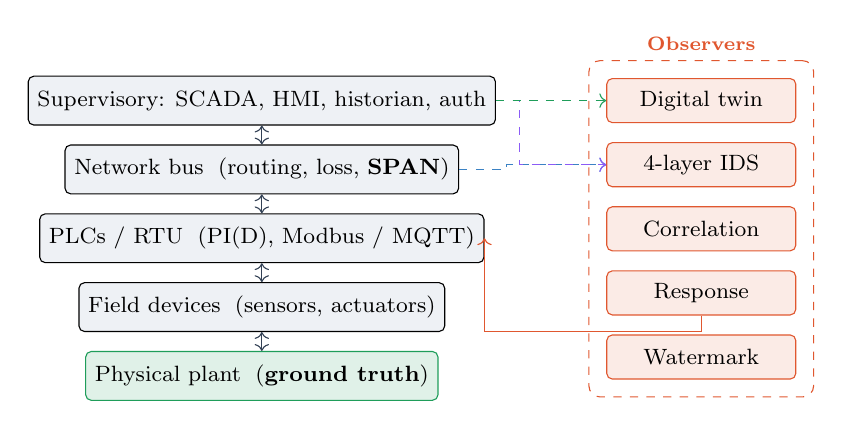
\begin{tikzpicture}[font=\footnotesize,node distance=2.4mm,
  layer/.style={draw,rounded corners=2pt,minimum width=42mm,minimum height=6.2mm,align=center,fill=lightgray},
  obs/.style={draw,rounded corners=2pt,minimum width=24mm,minimum height=5.6mm,align=center,fill=acc!12,draw=acc}]
\node[layer] (sup) {Supervisory: SCADA, HMI, historian, auth};
\node[layer,below=of sup] (net) {Network bus \;(routing, loss, \textbf{SPAN})};
\node[layer,below=of net] (plc) {PLCs / RTU \;(PI(D), Modbus / MQTT)};
\node[layer,below=of plc] (fld) {Field devices \;(sensors, actuators)};
\node[layer,below=of fld,fill=ltwin!14,draw=ltwin] (phy) {Physical plant \;(\textbf{ground truth})};
\draw[<->,slate] (sup)--(net); \draw[<->,slate] (net)--(plc);
\draw[<->,slate] (plc)--(fld); \draw[<->,slate] (fld)--(phy);
% observers on the right
\node[obs,right=14mm of sup] (twin) {Digital twin};
\node[obs,below=of twin] (ids) {4-layer IDS};
\node[obs,below=of ids] (corr) {Correlation};
\node[obs,below=of corr] (resp) {Response};
\node[obs,below=of resp] (wmk) {Watermark};
\begin{scope}[on background layer]
\node[draw=acc,dashed,rounded corners,fit=(twin)(wmk),inner sep=2.2mm,label=above:{\scriptsize\color{acc}\textbf{Observers}}] {};
\end{scope}
\draw[->,lnet,dashed] (net.east) -- ++(6mm,0) |- (ids.west);
\draw[->,lproc,dashed] (sup.east) -- ++(3mm,0) |- (ids.west);
\draw[->,ltwin,dashed] (sup.east) -- ++(9mm,0) |- (twin.west);
\draw[->,acc] (resp.south) -- ++(0,-2mm) -| (plc.east);
\end{tikzpicture}
\caption{Layered architecture. The attacker may touch only the network and the field devices; the twin, watermark, IDS and response engine observe the stack, and the response engine acts on simulated components.}
\label{fig:arch}
\end{figure}

Each 10\,Hz tick executes the fixed sequence of Fig.~\ref{fig:flow}. Four design invariants, enforced by automated tests, make the security evaluation meaningful: (i) the attacker can touch only the network and field-device firmware hooks---never the safety system, twin, IDS or watermark engine; (ii) the twin never reads ground-truth state; (iii) the safety system is independent of the network and the response engine; and (iv) ground-truth attack labels reach the evaluator only, never the detectors.

\begin{figure}[t]
\centering
\begin{tikzpicture}[font=\scriptsize,node distance=3.1mm,
  step/.style={draw,rounded corners=3pt,minimum width=58mm,minimum height=5.4mm,align=center,fill=lightgray},
  hot/.style={step,fill=acc!15,draw=acc},
  grn/.style={step,fill=ltwin!14,draw=ltwin},
  arr/.style={-{Stealth[length=2mm]},slate,thick}]
\node[hot] (s1) {1.\ Attack lab applies manipulations};
\node[grn,below=of s1] (s2) {2.\ Physical plant integrates (ground truth)};
\node[grn,below=of s2] (s3) {3.\ Hard-wired safety (SIS) may trip final elements};
\node[step,below=of s3] (s4) {4.\ Field I/O: sensors sample, PLCs scan};
\node[step,below=of s4] (s5) {5.\ Network bus delivers msgs \;(SPAN mirror)};
\node[step,below=of s5] (s6) {6.\ SCADA polling, historian \& twin feeds};
\node[step,below=of s6] (s7) {7.\ Digital twin + watermark update};
\node[step,below=of s7] (s8) {8.\ IDS (4 layers) $\rightarrow$ correlation};
\node[hot,below=of s8] (s9) {9.\ Response engine \;$\rightarrow$\; snapshot emitted};
\draw[arr] (s1)--(s2); \draw[arr] (s2)--(s3); \draw[arr] (s3)--(s4);
\draw[arr] (s4)--(s5); \draw[arr] (s5)--(s6); \draw[arr] (s6)--(s7);
\draw[arr] (s7)--(s8); \draw[arr] (s8)--(s9);
\end{tikzpicture}
\caption{Per-tick data-flow of the simulation engine (10\,Hz). Green steps read the true plant state; the attacker (step~1) and the SPAN-fed IDS (steps 5--8) never see it.}
\label{fig:flow}
\end{figure}

%=====================================================================
\section{Process and Network Simulation}
\textbf{Process model.} The primary plant is a lumped-parameter liquid-metal boiler with an intermediate heat exchanger (IHX), a secondary water loop and a turbine-generator (Fig.~\ref{fig:plant}). The bulk vessel temperature evolves as a heat balance:
\begin{equation}
C_b\,\frac{dT_b}{dt}=Q_{\text{heater}}-\dot{m}\,c_p\,(T_b-T_{\text{cl}})-UA_{\text{loss}}\,(T_b-T_{\text{amb}})
\end{equation}
The hot leg is a transport lag of the bulk temperature, the IHX uses a counter-flow effectiveness--NTU relation, and the secondary loop and generator follow first-order dynamics. Four auxiliary subsystems reuse the same abstractions: an induction motor (affinity-law current, winding temperature, vibration), a water-treatment plant (filtration fouling, turbidity, chlorine residual), a batch chemical-mixing reactor, and a pipeline/tank farm. Parameters are configurable and explicitly hypothetical.

\textbf{Field devices.} Each sensor turns the true value into a measurement via additive noise, quantisation and range clamping; each actuator applies a rate limit and first-order lag. Firmware hooks on these devices are the only point at which the attack laboratory can tamper with a field element.

\textbf{Control and safety.} Five controllers (four Modbus PLCs and one MQTT RTU) run PI(D) loops and sequencers. A separate Safety Instrumented System (SIS) reads the plant through its own instruments, is not attached to the network, and trips final elements \emph{after} any firmware tampering---so an emergency shutdown cannot be defeated by a compromised device.

\begin{figure}[t]
\centering
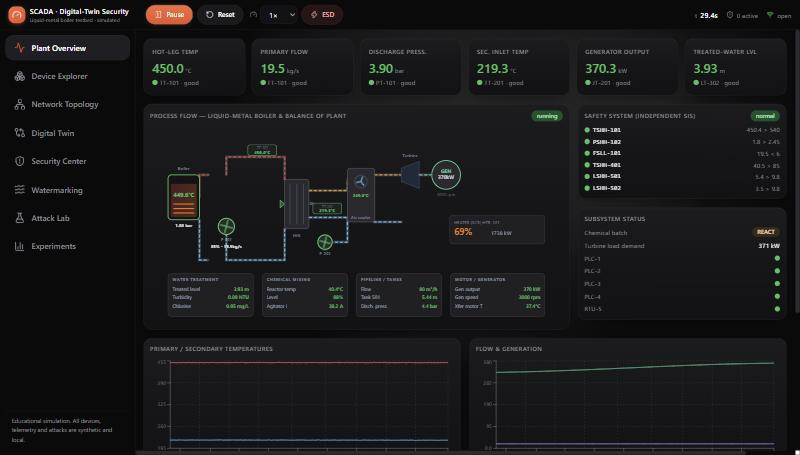
\includegraphics[width=\columnwidth]{figures/plant_overview.jpg}
\caption{Live operator HMI: the animated P\&ID of the liquid-metal boiler, balance-of-plant tiles, independent safety panel and live trend charts, all streamed at up to 10\,Hz over WebSocket.}
\label{fig:plant}
\end{figure}

\textbf{Network and protocols.} The network is a Purdue-zoned graph (supervisory L2, an industrial firewall, control L1, a cellular link to the remote RTU), shown in Fig.~\ref{fig:net}. Modbus~TCP is encoded and decoded as spec-conformant application data units (MBAP header plus PDU; function codes 03/04/06/16 and exceptions)~\cite{modbus}; OPC~UA and MQTT are modelled at the application level and labelled as such. A discrete-event bus carries every message with latency, jitter and loss, mirrors supervisory traffic to the IDS through a SPAN port, and supports man-in-the-middle interceptors used by the attack laboratory.

\begin{figure}[t]
\centering
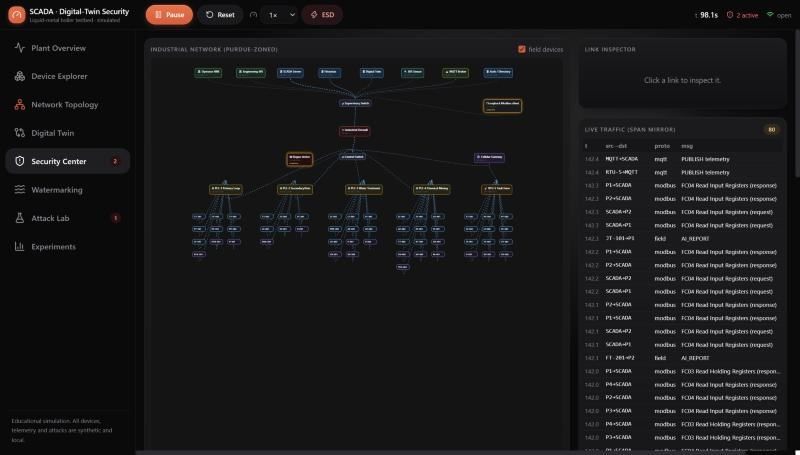
\includegraphics[width=\columnwidth]{figures/network_topology.jpg}
\caption{Interactive Purdue-zoned network: supervisory LAN, industrial firewall, control LAN with PLCs and field devices, a cellular gateway to the remote RTU, and the live SPAN-mirrored traffic (Modbus/MQTT) fed to the IDS.}
\label{fig:net}
\end{figure}

%=====================================================================
\section{Independent Digital Twin}
The digital twin is deliberately independent of the simulator. It integrates its own copy of the primary-loop physics with a fourth-order Runge--Kutta scheme and datasheet parameters that differ from the plant by a few percent (realistic model error). Its inputs are the commands the control system issued (plus the trusted watermark offset) and a small set of measured drivers---heater power, fan speed and generator load; it never reads the plant's hidden ground-truth state.

Each tick the twin forms a one-step-ahead prediction $\hat{y}_k$ and then applies a \emph{gated correction} toward each measurement $y_k$. The residual and its normalised innovation are:
\begin{equation}
r_k=y_k-\hat{y}_k,\qquad z_k=\frac{r_k-b_k}{\sigma_k}
\end{equation}
A measurement updates the corresponding state only if its innovation is inside the gate, $|z_k|<5$; readings that jump outside the gate are rejected. This is the key property: a falsified sensor cannot silently drag the twin along, so a stealthy lie produces a persistent, growing residual (Fig.~\ref{fig:twin}). Residuals feed a two-sided cumulative-sum (CUSUM) statistic for persistence and a counter for sudden errors, with an initial calibration window that estimates each residual's bias $b_k$ and spread $\sigma_k$.

\begin{figure}[t]
\centering
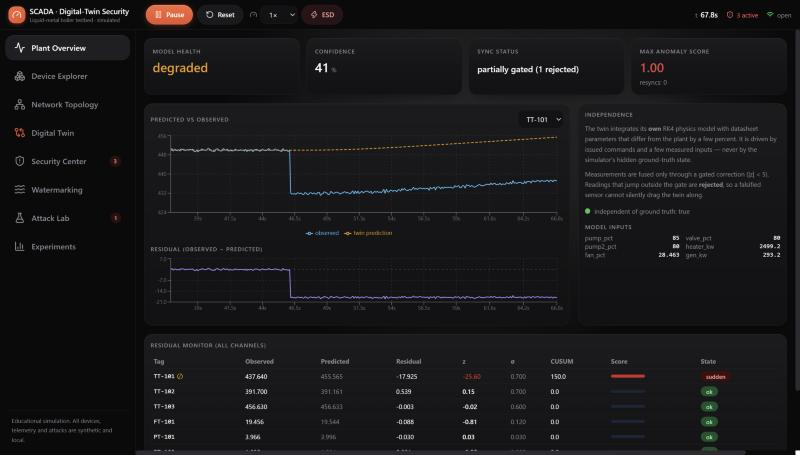
\includegraphics[width=\columnwidth]{figures/twin_divergence.jpg}
\caption{Twin view during a false-data injection on the hot-leg sensor. The observed value (blue) is pulled down to the falsified reading while the twin's independent prediction (orange) keeps tracking the real, rising temperature; the residual reaches $z=-25.6$ and model health degrades.}
\label{fig:twin}
\end{figure}

%=====================================================================
\section{Multi-Layer Intrusion Detection}
Detection is organised as four independent layers whose outputs are unified.
\begin{itemize}
\item \textbf{Network} (SPAN mirror only): rogue devices, MAC/ARP spoofing, unexpected flows, abnormal rates and floods, invalid Modbus sequences and byte-identical replays, unauthorised or out-of-envelope register writes, and policy violations.
\item \textbf{Process} (SCADA observations): alarm-limit violations, frozen (stuck-at) signals, implausible rate-of-change, setpoint deviation from the operator-approved value, pump-flow inconsistency, and energy-balance / analytical-redundancy violations.
\item \textbf{Digital twin}: persistent residuals, sudden prediction errors, and correlated multi-sensor anomalies, with a consistency test that separates falsification from an unmodelled change.
\item \textbf{Watermark}: the watermark decision (consistent / suspicious / inconclusive) as evidence.
\end{itemize}
Each detector emits \emph{conditions}; a finding manager deduplicates them into alert records. A correlation engine groups findings in the same zone and time window into incidents and combines per-layer confidence as
\begin{equation}
C=1-\prod_{\ell}\bigl(1-c_\ell\bigr),
\end{equation}
raising severity by one level per additional corroborating layer, classifying the incident with transparent rules, and recommending responses---without double-counting duplicate alerts (Fig.~\ref{fig:sec}).

\begin{figure}[t]
\centering

\includegraphics[width=\columnwidth]{figures/security_center.jpg}
\caption{IDS Security Center during a false-data injection: the alert feed (process energy-balance and twin sudden-residual evidence), the correlated critical incident at 96\% confidence, and the automatically executed responses with an incident timeline.}
\label{fig:sec}
\end{figure}

%=====================================================================
\section{Physical Watermarking}
The watermark engine injects a reproducible, bounded pseudo-random binary sequence (PRBS) into an eligible actuator command (by default the primary pump) inside the PLC's secured function block; the exported command register still reports the operator's base value. The excitation level for slot $k$ is a pure function of a seed and $k$, so the injector and the detector generate identical sequences without exchanging them over the network.

Two shadow copies of the twin's hydraulics are driven with and without the excitation; their difference is the \emph{expected} watermark response. SCADA telemetry (flow and discharge pressure), high-pass filtered, gives the \emph{observed} response. For each channel the detector computes the correlation $\rho$, the response gain relative to a calibrated baseline, and a signal-to-noise ratio, and returns one of three decisions: \textit{consistent}, \textit{suspicious}, or \textit{inconclusive}. Injection self-suspends on a safety trip, near actuator saturation, close to a process limit, or when measurement quality is poor, so the watermark never forces an unsafe perturbation and does not fabricate a result. In baseline operation the two channels show strong correlation ($\rho\approx0.80$ for flow and $\approx0.95$ for pressure); a replay that smooths away the injected signature is reported as suspicious.

%=====================================================================
\section{Attack Laboratory and Response}
Ten reproducible scenarios exercise the detectors: false sensor-data injection, frozen sensor readings, actuator-response manipulation, unauthorised setpoint modification, command replay, supervisory-link denial of service, out-of-policy engineering (insider) writes, digital-twin model tampering, watermark-observation interference, and a coordinated process-plus-network attack. Each scenario affects only simulated assets, records its seed and parameters, produces real changes in the simulation, exposes a ground-truth label, and supports stop/recover. Crucially, during telemetry falsification the physical process keeps evolving from the real actuator action while only the \emph{observed} values are altered---the gap the twin, the analytical redundancy and the watermark are designed to expose. Detection is driven purely by observed evidence.

A response engine operates in one of three modes: \textit{monitor} (record only), \textit{operator-approved} (confirm first), or \textit{automatic}. It acts through narrow, simulated effects: quarantine an endpoint, enable a PLC write allow-list, restore an approved setpoint, disable an account, mark a device suspicious, fail over to an authenticated anti-replay channel, enter a reduced-load safe state, resynchronise the twin, preserve evidence, or pause. The engine never issues real control and is kept separate from the safety interlocks.

%=====================================================================
\section{Experimental Methodology}
Experiments run a fresh, deterministic engine (master seed 1337) through a scripted timeline of baseline, attack and recovery phases, recording a per-sample trace of ground-truth labels, active findings (by layer and asset), setpoint deviation and incident state. The \emph{same} recorded trace is then scored under four detector configurations---network-only, network+process, network+process+twin, and the full stack with watermarking---so the comparison is strictly apples-to-apples on a single run. Each 2\,s evaluation window is labelled positive if the attack's effect was active for at least half of it and detected if a non-info finding mapped to the attacked zone during the window. From the confusion matrix we report precision, recall, the $F_1$ score, and detection latency. Ground-truth labels are consumed only by the evaluator, and every stochastic component draws from an independent seeded stream, so results replay exactly. The implementation ships with 56 automated tests.

%=====================================================================
\section{Results}
Table~\ref{tab:results} reports the detection $F_1$ of each configuration across the scenario suite. Fig.~\ref{fig:bars} isolates the two telemetry-falsification attacks, where a packet-only detector scores zero.

\begin{table}[t]
\centering
\caption{Detection $F_1$ by detector configuration (seed 1337, 2\,s windows). ``miss'' = no detection.}
\label{tab:results}
\renewcommand{\arraystretch}{1.18}
\setlength{\tabcolsep}{3.4pt}
\begin{tabular}{@{}lccccc@{}}
\toprule
\textbf{Scenario} & \textbf{Net} & \textbf{Net+} & \textbf{+Twin} & \textbf{Full} & \textbf{Lat.}\\
 & \textbf{only} & \textbf{Proc} & & \textbf{+WM} & \\
\midrule
A. Normal operation      & --   & --   & --   & --   & --\\
B. False data injection   & \textcolor{red}{miss} & 0.94 & 0.94 & \textbf{0.94} & 0.2\,s\\
C. Watermark interference & \textcolor{red}{miss} & \textcolor{red}{miss} & 0.71 & \textbf{0.96} & 1.1\,s\\
D. Unauthorised setpoint  & 0.91 & 0.91 & 0.91 & \textbf{0.91} & 0.0\,s\\
E. Command replay         & 0.93 & 0.93 & 0.93 & \textbf{0.93} & 0.5\,s\\
F. Coordinated            & 0.91 & 0.91 & 0.91 & \textbf{0.91} & 0.5\,s\\
\bottomrule
\end{tabular}
\end{table}

\begin{figure}[t]
\centering
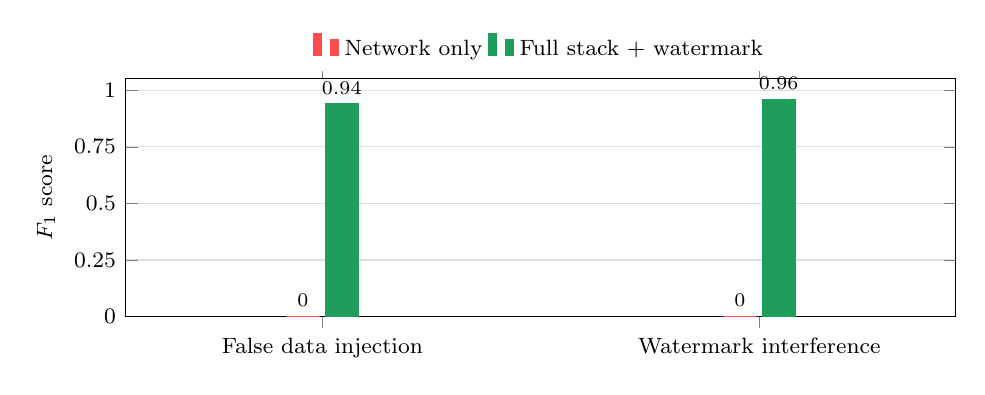
\begin{tikzpicture}
\begin{axis}[
  width=\columnwidth, height=46mm,
  ybar, bar width=12pt, enlarge x limits=0.45,
  ymin=0, ymax=1.05, ytick={0,0.25,0.5,0.75,1.0},
  ylabel={$F_1$ score}, ylabel style={font=\footnotesize},
  symbolic x coords={False data injection, Watermark interference},
  xtick=data, x tick label style={font=\footnotesize,align=center},
  tick label style={font=\footnotesize},
  legend style={font=\footnotesize,at={(0.5,1.03)},anchor=south,legend columns=2,draw=none},
  nodes near coords, nodes near coords style={font=\scriptsize},
  every node near coord/.append style={/pgf/number format/fixed,/pgf/number format/precision=2},
  ymajorgrids, grid style={gray!25},
]
\addplot[fill=red!70,draw=red!70] coordinates {(False data injection,0.0) (Watermark interference,0.0)};
\addplot[fill=ltwin,draw=ltwin] coordinates {(False data injection,0.94) (Watermark interference,0.96)};
\legend{Network only, Full stack + watermark}
\end{axis}
\end{tikzpicture}
\caption{On telemetry-falsification attacks a network-only IDS scores $F_1=0$, while the full multi-layer stack reaches $0.94$--$0.96$.}
\label{fig:bars}
\end{figure}

The results support four observations. (1)~\emph{No false positives in normal operation}: configuration~A raises no sustained alerts. (2)~\emph{Network-only is blind to telemetry falsification}: scenarios~B and~C produce no network-layer evidence and are missed by a packet-only detector; adding the process and twin layers recovers~B within $0.2$\,s. (3)~\emph{The watermark earns its place on~C}: the process layer alone sees nothing, the twin partially catches the slow drift ($F_1=0.71$), and adding the physical watermark raises detection to $0.96$. (4)~\emph{Command-path attacks are caught on the network}: unauthorised writes~(D), replay~(E) and the coordinated attack~(F) leave direct network evidence and are detected even by network-only, while the extra layers corroborate and classify them.

In a live run of scenario~B, the real hot-leg temperature continued to rise ($459.8\,^{\circ}$C) while SCADA displayed the falsified $442.3\,^{\circ}$C; the twin residual reached $z=-24.9$ with a saturated CUSUM, and the correlation engine raised a critical ``False data injection'' incident at 0.96 confidence, after which the automatic response quarantined the source, restored the setpoint and preserved evidence (Figs.~\ref{fig:twin},~\ref{fig:sec}). The plant returned to a healthy, synchronised state once the scenario was stopped.

%=====================================================================
\section{Discussion and Limitations}
The results make the central argument concrete: the detection layers are complementary, not redundant. Command-path attacks are visible on the network; telemetry-falsification attacks are invisible there but visible to a process-physics or twin-based detector; and an attacker who erases a passive signature can still be caught by an active watermark. A defender therefore needs all four, fused by correlation so that a coordinated attack---which no single layer sees in full---is still raised as one high-confidence incident.

The process model is a simplified, lumped-parameter abstraction with hypothetical parameters and is not a validated engineering or safety model. OPC~UA and MQTT are emulated at the application level rather than as wire-format protocols. The twin shares a model family with the plant (differing only in parameters), so a sufficiently slow, in-gate ramp can still bias it; the watermark and redundancy checks are the intended mitigations, and quantifying the stealthy-ramp detection boundary is future work. The evaluation uses a single seed per scenario; a broader stochastic study would tighten the metrics.

%=====================================================================
\section{Conclusion}
We presented a self-contained, reproducible cyber-physical security testbed that couples a simulated SCADA plant with an independent digital twin, a four-layer intrusion detection system, a physical-watermarking engine, an attack laboratory and an automated response engine, all running live at 10\,Hz with an operator HMI. Across ten reproducible attacks we showed quantitatively that network-only detection is blind to telemetry falsification while the multi-layer stack detects it within fractions of a second, and that the physical watermark adds detection value precisely where passive layers fail. Future work includes characterising the stealthy in-gate ramp boundary, adding learning-based detectors alongside the transparent rules, broadening the stochastic evaluation, and binding real protocol libraries over an isolated loopback network.

%=====================================================================
\begin{thebibliography}{00}
\bibitem{stuxnet} N. Falliere, L. O. Murchu, and E. Chien, ``W32.Stuxnet Dossier,'' Symantec Security Response, 2011.
\bibitem{mo2009} Y. Mo and B. Sinopoli, ``Secure control against replay attacks,'' in \textit{Proc. 47th Allerton Conf.}, 2009, pp. 911--918.
\bibitem{mo2015} Y. Mo, S. Weerakkody, and B. Sinopoli, ``Physical authentication of control systems,'' \textit{IEEE Control Syst. Mag.}, vol. 35, no. 1, pp. 93--109, 2015.
\bibitem{cardenas} A. A. C\'ardenas \textit{et al.}, ``Attacks against process control systems: Risk assessment, detection, and response,'' in \textit{Proc. ACM ASIACCS}, 2011, pp. 355--366.
\bibitem{urbina} D. Urbina \textit{et al.}, ``Limiting the impact of stealthy attacks on industrial control systems,'' in \textit{Proc. ACM CCS}, 2016, pp. 1092--1105.
\bibitem{swat} J. Goh, S. Adepu, K. N. Junejo, and A. Mathur, ``A dataset to support research in the design of secure water treatment systems,'' in \textit{Proc. CRITIS}, 2016.
\bibitem{minicps} D. Antonioli and N. O. Tippenhauer, ``MiniCPS: A toolkit for security research on CPS networks,'' in \textit{Proc. ACM CPS-SPC}, 2015, pp. 91--100.
\bibitem{ukraine} R. M. Lee, M. J. Assante, and T. Conway, ``Analysis of the cyber attack on the Ukrainian power grid,'' E-ISAC/SANS, 2016.
\bibitem{modbus} Modbus Organization, ``Modbus Application Protocol Specification V1.1b3,'' 2012.
\bibitem{eckhart} M. Eckhart and A. Ekelhart, ``Towards security-aware virtual environments for digital twins,'' in \textit{Proc. ACM CPSS}, 2018, pp. 61--72.
\end{thebibliography}

\end{document}
